\section{Abstract}
Genetic diversity in animal immune systems is usually beneficial. In hybrid recombinants, this is less clear, as the immune system could also be impacted by genetic conflicts. In the European house mouse hybrid zone, the longstanding impression that hybrid mice are more highly parasitized and less fit than parentals persists despite the findings of recent studies. Working across a novel transect we assessed infections by intracellular protozoans, \textit{Eimeria} spp., and infections by extracellular macroparasites, pinworms. For \textit{Eimeria} we found lower intensities in hybrid hosts than in parental mice but no evidence of lowered probability of infection or increased mortality in the centre of the hybrid zone. This means ecological factors are very unlikely to be responsible for the reduced load of infected hybrids. Focusing on parasite intensity (load in infected hosts) we also corroborated reduced pinworm loads reported for hybrid mice in previous studies. We conclude that intensity of diverse parasites, including the previously unstudied \textit{Eimeria}, is reduced in hybrid mice compared to parental subspecies. We suggest caution in extrapolating this to differences in hybrid host fitness in the absence of, for example, evidence for a link between parasitemia and health.

\textbf{Keywords: parasites, hybridization, resistance}

\section{Introduction}
The relevance of hybridization, producing individuals admixed between genetically distinct populations, is increasingly recognized by biologists. \cite{mallet_hybridization_2005} suggested that hybridization occurs in more than 10\% of animal species and 25\% of vascular plant species. Recently, the realization that humans are also a product of hybridization has raised interest further \citep{green_draft_2010}. In a conservation context hybridization with introduced species can threaten autochthonous endangered animals \citep{simberloff_hybridization_1996}. Parasites are omnipresent in natural systems and impact human and animal health \citep{schurer_community-based_2016}. It is therefore important for biologists to comprehend the interplay between parasites and hosts under hybridization.
\par The European house mouse hybrid zone (HMHZ), one of the first animal hybrid zones studied for differences in parasite loads \citep{sage_wormy_1986}, is a tension zone characterized by selection against hybrids replaced by immigrating less admixed mice \citep{barton_analysis_1985}. After ~500 000 years of (mostly) allopatric divergence two house mouse subspecies, \textit{Mus musculus domesticus} and \textit{Mus musculus musculus} (hereafter Mmd and Mmm), have come into secondary contact in Europe as a result of different colonization routes south and north of the Black Sea, respectively \citep{boursot_evolution_1993, duvaux_isolation_2011}. The HMHZ is about 20 km wide and more than 2500 km long, running from Scandinavia to the coast of the Black Sea \citep{baird_what_2012, boursot_evolution_1993, jones_norwegian_2010, macholan_location_2003}. This zone represents a semi-permeable barrier to gene flow between the two taxa \citep{macholan_genetic_2007, macholan_assessing_2011}. The main selective forces acting against hybrids are thought to be endogenous rather than ecological \citep{baird_what_2012, boursot_evolution_1993}, for example disruption of spermatogenesis in hybrids \citep{albrechtova_sperm-related_2012, turner_reduced_2012}.
\par Hybrids in tension zones have reduced fitness compared to individuals with “parental” genotypes due to genetic incompatibilities revealed on parentals’ secondary contact \citep{barton_analysis_1985}. As different components of fitness can vary independently, the immune system of hybrids might either benefit from recombinant genetic heterogeneity or suffer from incompatibilities. In the case of benefit we might expect decreased parasite load in hybrid individuals; in the case of incompatibilities we might expect increased load in hybrid individuals, compared to parental hosts. Parasites are traditionally seen as decreasing their hosts’ fitness, and differences in resistance to parasites between hybrid and pure hosts were suggested to affect the dynamics of hybrid zones \citep{fritz_resistance_1999}. An involvement of parasites in the maintenance or breakdown of species barriers, however, has never been clearly justified or demonstrated \citep{baird_shifting_2019}. In the HMHZ system, there is disagreement on both the direction of effects of hybridization on parasites \parencites[see][vs]{sage_wormy_1986, moulia_wormy_1991}{baird_where_2012} and on the interpretation of these findings with regards to host fitness and hybridization \parencites[see for example][]{theodosopoulos_parasites_2019, baird_shifting_2019}.
\par Initial results on parasites obtained in the HMHZ and experimental studies seemed to indicate elevated parasite loads in hybrids. This has been interpreted as potentially leading to fitness reductions in hybrids, hampering hybridization and thus reinforcing species barriers \citep{moulia_wormy_1991, moulia_experimental_1993, sage_wormy_1986}. Infection experiments using the protozoan Sarcocystis muris led to a similar conclusion \citep{derothe_susceptibility_2001}. Other laboratory experiments, however, showed either no effect in inter-subspecies F1s on helminth load or even reduced load in inter-subspecies F1s compared to pure mouse strains \citep{derothe_recombination_2004, moulia_hybrid_1995}. In 2012, more than two decades after the original field studies \citep{moulia_wormy_1991, sage_wormy_1986}, Baird et al. found, (with much larger sample size, clearer sampling design and more up to date inference), reduced helminth loads in hybrid mice \citep{baird_where_2012}, especially for the pinworms \textit{Aspiculuris tetraptera} and \textit{Syphacia obvelata} and the whipworm \textit{Trichuris muris}. It should be noted that the design of the field studies preceding the \cite{baird_where_2012} reappraisal usually suffered from low sample sizes and/or maintenance of mice under laboratory conditions before assessment of parasite burden, which may have allowed spurious signal to dominate the results. Nevertheless, even the basic direction of parasite load differences in hybrid mice compared to parental genotypes still seems controversial to some researchers. 
\par We now see that, despite working within the framework of the same hybrid zone, two different interpretations of parasite loads in hybrid mice have arisen. It should be noted that all the previous studies chose to focus on either helminth or protozoan parasite models. In vertebrates, the immune mechanisms of parasite control differs greatly between these two groups. Extracellular macroparasites like helminths trigger a T helper type 2 (Th2) -dominated response, and intracellular microparasites like protozoa trigger a T helper type 1 (Th1) -mediated response \citep{sher_regulation_1992}. One way forward in such circumstances is to test hypotheses over replicates and “along different axes” of parasitism, and to consider simultaneously helminths and protozoans to address the generality of hybrid response. To distinguish between interpretations of parasite load we here asked if (1) parasite loads are higher or lower in hybrids compared to parentals, and (2) if these loads are consistent, or differ, between prevalent representative helminths and protozoa. We did so in a geographically new transect replicate of the HMHZ.
\par Pinworms (oxyurids) have been detected in mice in numerous field studies \parencites[see for example][]{behnke_aspiculuris_1975, behnke_aspiculuris_1976,kriska_parasitic_1993, ressouche_host_1998}. They have been shown to be the most prevalent helminths infecting house mice in the HMHZ \citep{gouy_de_bellocq_new_2012}. They are often considered to provoke mild symptoms on their hosts, even if in rare conditions (e.g. particularly high burden) they have been shown to affect the health of laboratory mice \citep{taffs_pinworm_2016}. \textit{Eimeria} spp. are often considered host-specific, with several thousand species parasitizing different vertebrates \citep{chapman_chapter_2013, haberkorn_entwicklung_1970}. These parasites infect the intestinal epithelial cells of vertebrates and induce symptoms such as weight loss and diarrhoea. For example, infecting the NMRI mouse laboratory strain with \textit{Eimeria} oocysts isolated from mice captured in the HMHZ resulted in a weight loss up to 20\% compared to control \citep{al-khlifeh_eimeria_2019}. In the European HMHZ, three \textit{Eimeria} species have been identified: \textit{E.~ferrisi} , \textit{E.~falciformis} , and \textit{E. vermiformis}  with prevalences of 16.1\%, 4.2\% and 1.1\%, respectively \citep{jarquin-diaz_detection_2019}. 
\par We assessed \textit{Eimeria} infection in a novel transect of the HMHZ in Brandenburg, northeastern Germany, in which the hypothesis of hybrid resistance/susceptibility to parasite had never before been tested. We assessed the impact of host hybridization on intensity of this parasite. By focusing on parasite intensity \parencite[extent of parasite infection in only infected animals;][]{bush_parasitology_1997}, we arguably exclude ecological factors for differences in load. We show that (1) parasite loads are consistently lower in hybrids compared to parental genotypes in the HMHZ and (2) that this pattern is similar for our intracellular and extracellular parasite models.

\section{Material \&  Methods}
\subsection{Sampling}
Our sampled individuals consist of 660 house mice trapped using live traps placed in farms or houses between 2014 and 2017. The study area ranges from 51.68 to 53.29 degrees of latitude (200 km) and from 12.52 to 14.32 degrees of longitude (140 km). Each year mice were trapped in September when it is possible to capture a high number of mice in this region. In addition, sampling at the same season every year reduces potential seasonal variation \citep{abu-madi_seasonal_2000, haukisalmi_population_1988}. The locations for trapping were selected across a geographical range allowing both parental and hybrid/recombinant individuals to be captured. Mice were individually isolated in cages and then euthanized by isoflurane inhalation followed by cervical dislocation within 24 hours after capture (animal experiment permit No. 2347/35/2014). Individual mice were measured (body length from nose to anus), weighted, and dissected. Tissue samples (muscle and spleen) were transported in liquid nitrogen and stored at -80°C for subsequent host genotyping. Digestive tracts were dissected and inspected for helminth parasites (see below). Ileum, caecum and colon tissues were frozen in liquid nitrogen and then stored separately at -80°C. A median of 2 mice per locality were captured. A table of individual mouse data including hybrid indices, georeferences and parasite loads is available in Supplementary Table S3. To investigate \textit{Eimeria} infections we checked 384 mice sampled in 2016 and 2017 for the presence and intensity of tissue stages (\textbf{Figure 2.2a}). Between 2014 and 2017, 585 mice were investigated for helminths (\textbf{Figure 2.3a}). 

\subsection{Host genotyping}
The admixture of mouse genomes across the HMHZ was estimated for each mouse as a value of the hybrid index (HI) calculated as a proportion of Mmm alleles in a set of 14 diagnostic markers. This set consists of one mitochondrial marker \parencite[BamHI, a restriction site in the Nd1 gene;][]{bozikova_mitochondrial_2005, munclinger_genetic_2002} one Y-linked marker \parencite[presence/absence of a short insertion in the Zfy2 gene;][]{boissinot_discordant_1997, nagamine_musculus-type_1992}, six X-linked markers (three B1 and B2 short interspersed nuclear elements in Btk, Tsx \citep{munclinger_b1_2003}, and Syap1 \citep{macholan_genetic_2007}, X332, X347 and X65 \citep{dufkova_inference_2011, dureje_mouse_2012}), and six autosomal markers \parencite[Es1, H6pd, Idh1, Mpi, Np, Sod1;][]{macholan_genetic_2007}. HIs ranged from 0 to 1, HI of 0 indicating a pure Mmd and HI of 1 a pure Mmm \citep{baird_what_2012, macholan_genetic_2007}. At least 10 loci provided information for 92\% of the mice, and at least 4 loci for the remaining 8\% due to technical issues. Histograms for the number of genotyped markers, as well as their distribution across the hybrid index indicate no bias in genotyping (\textbf{Supplementary Figure S2.1}). 
\par The expected centre of the HMHZ across the study area was estimated using the program Geneland v4.0.8 (with graphical resolution increased over defaults, the modified code is available at \url{https://github.com/alicebalard/Geneland} as a complete R-package), based on a subset of the six autosomal markers that were genotyped in all individuals with 6 diploid markers (N=598 mice). Geneland uses a Markov chain Monte Carlo (MCMC) approach to combine both geographical and genetic information \citep{guillot_geneland_2005}. The number of clusters was set to 2, 106 MCMC iterations were performed and saved every 100th iterations (104 iterations saved). The first 200 iterations were discarded as burn-in and the resolution of the map was set to 2000 pixels for the x axis and 1400 for the y axes corresponding roughly to 1 pixel for 100m \citep{macholan_assessing_2011}.

\subsection{Parasite load estimation}
Mouse digestive tracts were dissected and inspected for helminth presence with a binocular microscope. Helminths were counted and stored in 70\% ethanol for later identification by molecular analysis and, when more than one worm per host was present, in 3.5\% formalin for later morphological comparison with species descriptions. As in this study we required high statistical power to test our hypotheses, we considered only the most prevalent helminths, the oxyurids \textit{Syphacia obvelata} and \textit{Aspiculuris tetraptera}. Histograms presenting the distribution of  counts for other helminths can be found in \textbf{Supplementary Figure 2.S2} and data is available in \textbf{Supplementary Table S2.3}.

\par 
DNA was extracted from ileum and caecum tissues and quantitative PCR (qPCR) was used for estimation of \textit{Eimeria} spp. load. DNA extraction was performed using the innuPREP DNA Mini Kit (Analytik Jena AG, Jena, Germany) following the instructions of the manufacturer with additional mechanical tissue disruption with liquid nitrogen in a mortar. Both quality and quantity of isolated DNA were measured by spectrophotometry in a NanoDrop 2000c (Thermo Scientific, Waltham, USA). The presence of \textit{Eimeria} spp. was tested using qPCR to detect intracellular stages of the parasite as well as a house mouse house-keeping gene as internal reference. Primers used for \textit{Eimeria} spp. detection targeted a short mitochondrial COI region (Eim\textunderscore COI\textunderscore qX-F:  TGTCTATTCACTTGGGCTATTGT; Eim\textunderscore COI\textunderscore qX-R: GGATCACCGTTAAATGAGGCA), while \textit{Mus musculus} primers targeted the CDC42 nuclear gene \parencite[Ms\textunderscore gDNA\textunderscore CDC42\textunderscore F: CTCTCCTCCCCTCTGTCTTG; Ms\textunderscore gDNA\textunderscore CDC42\textunderscore R: TCCTTTTGGGTTGAGTTTCC; ][]{al-khlifeh_eimeria_2019, jarquin-diaz_detection_2019}.
\par These qPCRs have been independently confirmed with respect to detection of experimental infection \citep{al-khlifeh_eimeria_2019} and with genotyping PCRs using different primers and markers \citep{jarquin-diaz_detection_2019}. Reactions were performed using 1X iTaqTM Universal SYBR® Green Supermix (Bio-Rad Laboratories GmbH, München, Germany), 400 nM of each primer and 50 ng of DNA template in 20 µL final volume. Cycling amplification was carried out in a Mastercycler® RealPlex 2 thermocycler (Eppendorf, Hamburg, Germany) with the following amplification program: 95°C initial denaturation (2 min) followed by 40 cycles of 95°C denaturation (15 s), 55°C annealing (15 s) and 68°C extension (20 s). Melting curve analyses were performed in order to detect primer dimer formation and unspecific amplification. ΔCt was calculated as difference of the threshold cycle (Ct) between mouse and \textit{Eimeria} spp. values (corresponding to a log2 ratio between parasite and mouse DNA). This method was validated in an infection experiment of NMRI mice \citep{al-khlifeh_eimeria_2019}. We considered ΔCt = -5 our limit of detection as at this limit it was possible to obtain genotyping data for all samples using independent PCR reactions \citep{ahmed_novel_2019, jarquin-diaz_detection_2019}. Samples with a ΔCt lower than -5 were considered negative (unspecific signal due to amplification of non-target DNA). Samples with a ΔCt higher than -5 for at least one of the two intestinal tissues were considered positive, and in the case of detection in both tissues, the higher value was taken as a proxy of individual parasite load. This parasite load of the intestinal tissue stage is denoted as “ΔCtMouse−\textit{Eimeria}” throughout the following. \textit{Eimeria} identification at the species level was performed by means of two PCR markers (18S and COI) followed by a confirmation of morphology and tissue preference as described in \cite{jarquin-diaz_detection_2019} (column “eimeriaSpecies” of \textbf{Supplementary Table S2.3}).

\subsection{General parasite assessment}
As the distributions of parasite loads are expected to be highly skewed \citep{bliss_fitting_1953}, the median (as an estimator for the mode) is more informative than the mean \citep{rozsa_quantifying_2000}. We therefore report the median of parasite load across all hosts (median abundance) and of parasite load of infected host (median intensity) for pinworms, and only median intensity for \textit{Eimeria} spp. For qPCR some uninfected samples present technical noise due to unspecific amplification of non-target DNA. We therefore used a qPCR threshold validated by independent genotyping PCRs \parencite[see “Fig. 4” of][]{jarquin-diaz_detection_2019} to establish the infection status of each sample \parencite[and we do not report abundance for \textit{Eimeria}, see][for details]{jarquin-diaz_detection_2019}. Prevalence (relative frequency of infected individuals amongst all tested individuals) confidence intervals were obtained with Sterne’s exact method \citep{reiczigel_exact_2010, sterne_remarks_1954}. Calculations were performed using the epiR package \citep{nunes_epir_2018} running within the R statistical computing environment \citep{R_2010}.

\subsection{Statistical design: testing hybrid resistance/susceptibility in a natural system}
According to the SIR model of epdidemiology, individuals can be divided into susceptible (S), infected (I), and removed (R, dead or recovered). Animals captured in the field can show (1) absence, or (2) presence of a given parasite. Absence of a parasite in a given host can result from absence of exposure to the parasite, complete host resistance, recovery, or death \citep{kramer_modern_2010}. On the other hand, quantitative parasite load depends on intrinsic host or parasite components or their interactions. We argue that when testing the hypotheses of hybrid resistance or susceptibility in a natural system, a focus on the latter is beneficial. Therefore, we test a potential increase or decrease of parasite load in infected animals (intensity) towards the centre of the zone compared to its sides. We performed this analysis for our parasites of interest, but first verified that we could exclude differences in prevalence (probability of infection) across the hybrid index for each parasite. This leaves mortality as the only epidemiological factor (in the SIR model) to potentially influence both prevalence and intensity, we therefore additionally tested increased mortality by analyzing differences in (infected/uninfected) age categories across the hybrid index (see below: Statistical test for different mortality of hybrids). 
\par The hybridization level in each individual was modelled as the degree to which new gene combinations are brought together compared to the pure subspecies. This was estimated from the hybrid index using the function for expected heterozygosity \citep{baird_where_2012}: 

\[He = 2 · HI · (1 − HI) ,           (Eq. 1)\]

\subsection{Statistical prediction of probability of infection by parasites along the hybrid zone}
We considered the predicted probability of infection across the HI as equivalent to the prevalence and modelled a dichotomous response variable (uninfected = 0; infected = 1) by logistic regression. We performed two analyses, one testing for prevalence differences on both halves of the hybrid index separately and a second one with a unified “genetic distance to zone centre” (for individuals with HI between 0 and 0.5 the proxy is HI, for individuals with HI between 0.5 and 1 the proxy is 1 – HI). This means we do not blindly assume equality of prevalence at both ends of the hybrid index, but also maximize power to reject the null hypothesis (esp. in case of a negative result in the separate analysis). Analyses were done in R with the function glm from the stats package \citep{R_2010} including host sex and interaction terms with the variable representing hybrid genetics.

\subsection{Statistical test for different mortality of hybrids}
Secondly, morbidity or mortality caused by hyperparasitism could impact both prevalence and intensity measures of parasite loads, as only the surviving, less parasitized mice could be captured. This, however, would also lead to differences in age distribution along the hybrid index. We used an age estimation based on weight \parencite[as in][]{behnke_aspiculuris_1976} as a proxy to test if hybrid mice were younger or older than that expected for intermediate between pure hybridizing taxa (“additivity”). Values of body weight are well described by the normal distribution, parameterized by its standard deviation (allowed to vary freely during maximum likelihood searches) and its mean defined as:

\[ExpectedBodyWeight = (BW1 + (BW2 − BW1) · HI) · (1 − alpha · He) ,     (Eq. 2)\]
where BW1 is the expected body weight of pure Mmd, BW2 the expected body weight of pure Mmm. Alpha represent the hybridization effect, or deviation from additivity between the two parental genomes. We allowed difference between sex and taxa, fit the models using maximum likelihood \parencite[using the R package mle2;][]{bolker_bbmle_2017}, either including or excluding the hybridization effect parameter (by setting HI = 0 in ExpectedBodyWeight), and we compared these two models using the G-test. 

\subsection{Statistical test of the host hybridization effect on parasite intensity}
It has been shown that macroparasites tend to aggregate within their hosts, the majority of host carrying no or a low burden, and a minority a high one \citep{shaw_patterns_1995}. We modelled this distribution of parasite burden in infected hosts as negative binomial. Following the approach of \cite{baird_where_2012}, we tested if hybrid mice had higher or lower parasite burdens than that expected in case of additivity (if the relationship between host parasite load and hybrid index was linear). 
\par The parasite load for a given HI was then estimated as follows:

\[ExpectedLoad = (L1 + (L2 − L1) · HI) · (1 − alpha · He) ,           (Eq. 3)\]
where L1 is the parasite load of pure Mmd, L2 the parasite load of pure Mmm, and alpha the hybridization effect (deviation of parasite estimated load from the additive model). We considered four nested hypotheses increasing in complexity, and compared them with the G-test (likelihood ratio test) to consider a more complex hypothesis only when justified by a significant increase in likelihood. Expected parasite load is fixed to be identical for both subspecies and both host sexes in hypothesis H0. The more complex H1 allows load differences for the host sexes, H2 allows different loads between the subspecies at the extremes of the hybrid index, and H3 allows differences both between the subspecies and sexes.
\par Adequate distributions of values for each parasite and detection method considered were selected using log likelihood and AIC criteria and by comparing goodness-of-fits plots (density, CDF, Q-Q, P-P) (R packages MASS \citep{venables_modern_2002} and fitdistrplus \citep{delignette-muller_fitdistrplus_2015} (see \textbf{Supplementary Figure S2.4}). The negative binomial distribution should perform well for macroparasite counts \citep{crofton_quantitative_1971, shaw_patterns_1995}, which was confirmed for helminths in another, geographically distinct, transect \citep{baird_where_2012}. Values of (ΔCtMouse−\textit{Eimeria}) were found to be well described by the Weibull distribution after being positively shifted. 
\par The negative binomial distribution is parameterized by two arguments: its expectation (Expected Load, Eq. 3), and the inverse of its aggregation, which is allowed to vary across HI as:

\[Aggregation = (A1 + (A2 − A1) · HI) + Z · He ,           (Eq. 4)\] 
Z being the deviation from the additive model, in proportion to He, which is maximal in the zone centre \citep{baird_where_2012}. The Weibull distribution is parametrized by its shape and scale parameters (allowed to vary freely during maximum likelihood search) linked by the formula:

\[Scale = ExpectedLoad / Ⲅ (1 + 1/ shape) ,           (Eq. 5)\]
Ⲅ  being the gamma function. 
\par We fit the models using likelihood maximization \parencite[using the R package mle2;][]{bolker_bbmle_2017}. Parasite load was estimated either including or excluding the hybridization effect parameter (by setting HI = 0 in ExpectedLoad), and we compared these two models using the G-test. In the case of ΔCtMouse−\textit{Eimeria}, the Weibull distribution requires positive values as input. Therefore, we estimated an extra “shift parameter” which was optimized by maximum likelihood.

\subsection{Test of body condition differences between infected and non-infected mice across the hybrid zone}
After the previous tests on hybrid resistance/susceptibility to parasites, we wanted to see if our field system could allow differences in tolerance to parasites to be tested. We thus tested whether we could detect different body condition between infected and non-infected mice along the hybrid index. Residuals from ordinary least squares regression of body weight by body length were estimated for each individual, separately for males and females. Pregnant females were excluded from the analysis. Individuals with a positive residual were considered in better condition than individuals with a negative one, as this index correlates with variation in fat, water, and lean dry mass \citep{schulte-hostedde_restitution_2005}. We tested if hybrid mice had higher or lower residuals than that expected for intermediate between pure hybridizing taxa (“additivity”), and if the potential hybridization effect was different between infected and not infected mice, for \textit{Eimeria} spp. as well as for pinworm infections. Differences between the loads of the pure parental subspecies on each side of the hybrid zone were allowed.
\par Values of residuals of body weight by body length regression are well described by the normal distribution, parameterized by its standard deviation (allowed to vary freely during maximum likelihood searches) and its mean defined as:

\[ExpectedResidual = (R1 + (R2 − R1) · HI) · (1 − alpha · He) (Eq. 6) \]

where R1 is the expected residual value of pure Mmd, R2 the expected residual value of pure Mmm, and alpha the hybridization effect. We fit the models using maximum likelihood \parencite[using the R package mle2;][]{bolker_bbmle_2017}, either including or excluding the hybridization effect parameter (by setting HI = 0 in ExpectedResiduals), and we compared these two models using the G-test. 
\par All graphics were produced using the R packages ggplot2 \citep{wickham_ggplot2_2016} and ggmap \citep{kahle_ggmap_2013}, and compiled using the free software inkscape v.0.92 (\url{https://inkscape.org}). Full R code used for this article can be found at:	 \url{https://github.com/alicebalard/Article\textunderscore IntensityEimeriaHMHZ/tree/master/code}

\section{Results}
\subsection{Host genotyping and characterization of the HMHZ for a novel transect}
We caught and genotyped a total of 650 mice (359 females, 291 males) over four sampling seasons (2014: N=86; 2015: N=156; 2016: N=167; 2017: N=241) at 149 localities. On the probability map of the hybrid zone centre, shown in \textbf{Figure 2.1}, we see that the HMHZ runs across the former East Germany, making a broad arc around the city of Berlin, approaching within ca. 20 km of the bordering Oder River near Eberswalde. 

\begin{figure}[H]
    \centering
    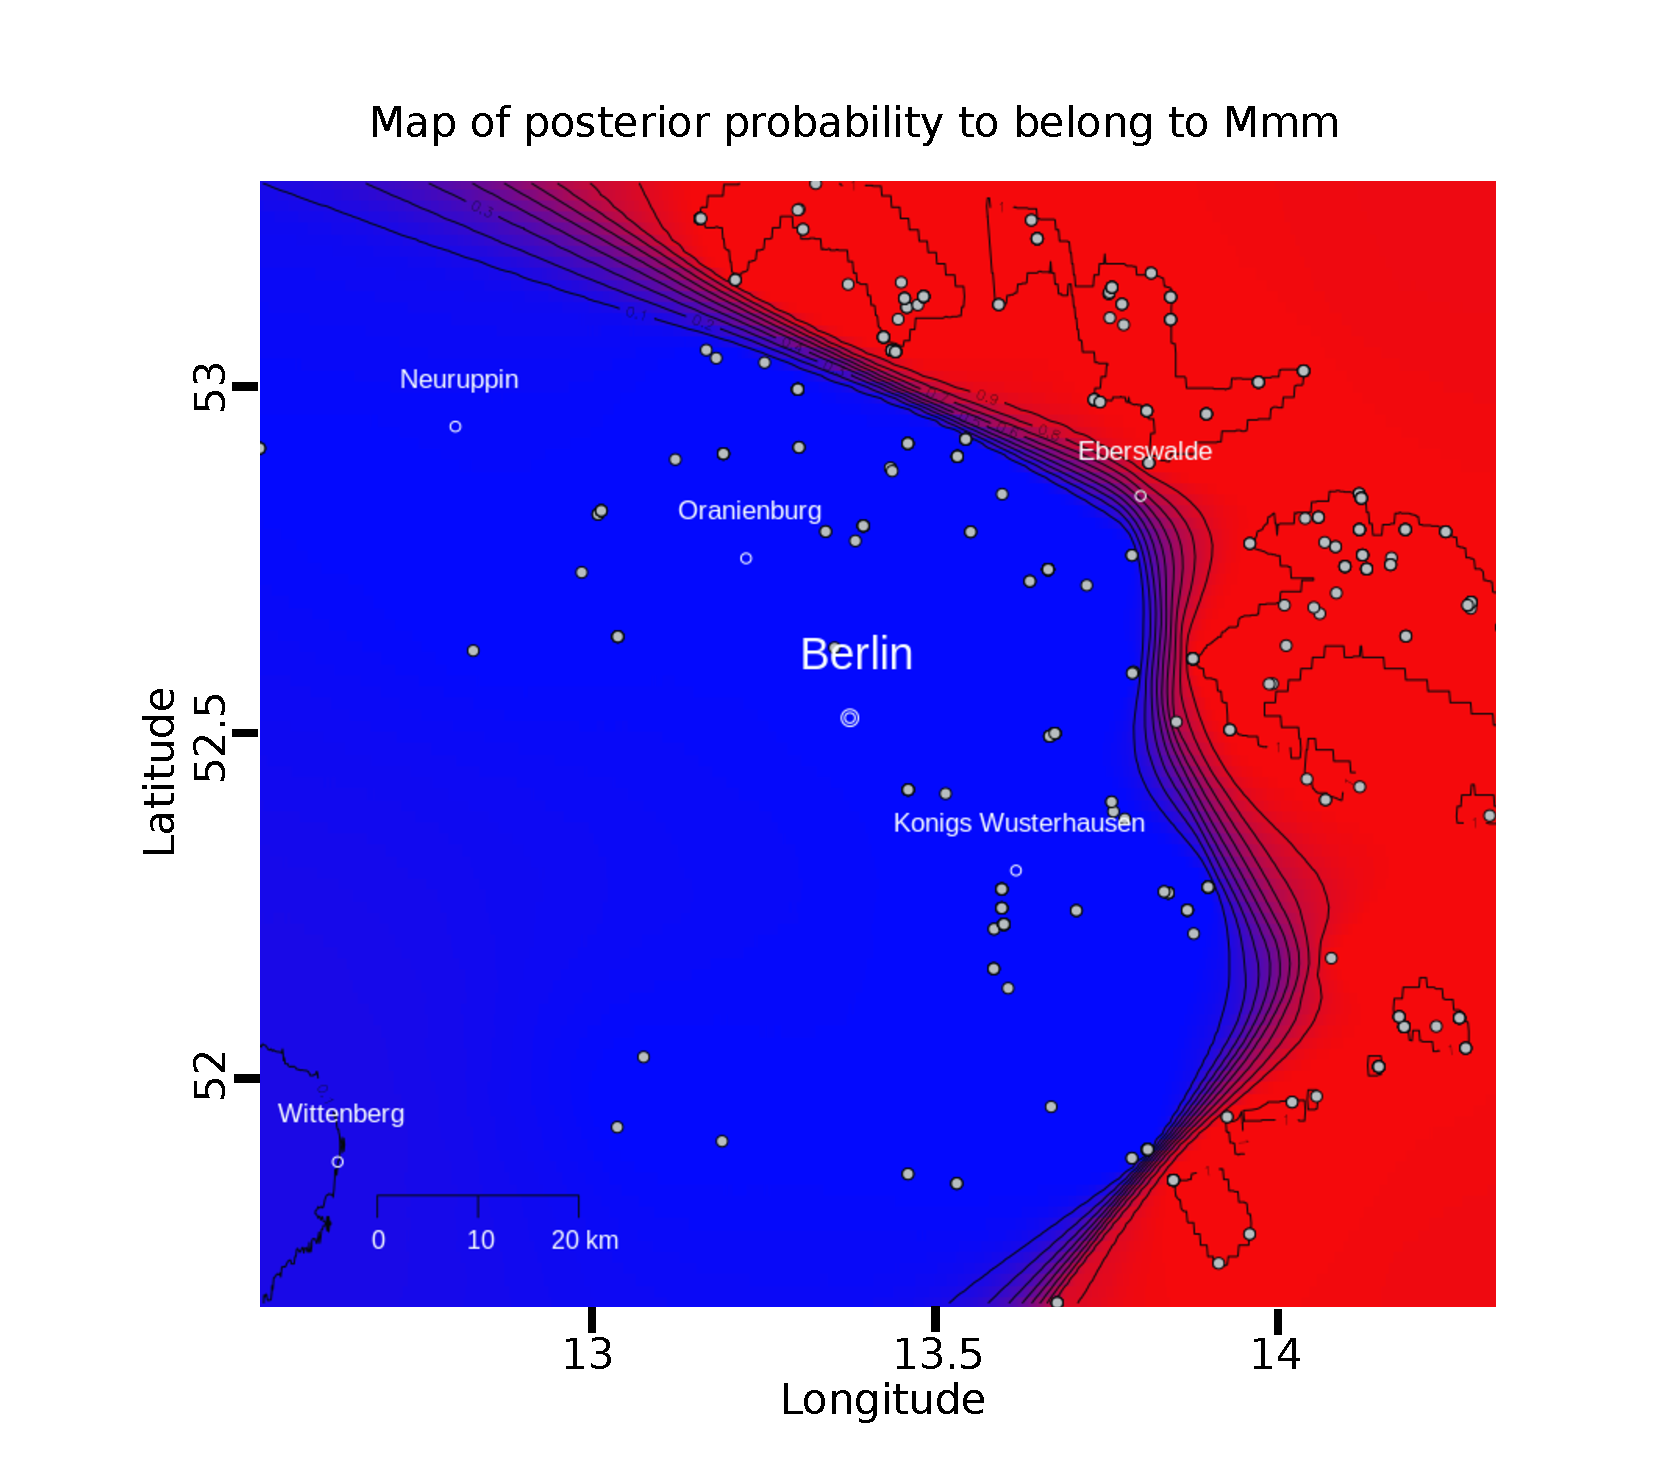
\includegraphics[width=\linewidth,height=\textheight,keepaspectratio]{images/2article1/Figure1.pdf}
    \caption{\textbf{Geographic range of house mouse subspecies in the European house mouse hybrid zone}. Spatial organization of the HMHZ was inferred using all individuals with 6 autosomal markers available (N=598 mice) (Es1, H6pd, Idh1, Mpi, Np, Sod1). \textit{Mus musculus domesticus} is found west of the hybrid zone (blue), \textit{Mus musculus musculus} east of it (red). The numbers at the level contours indicate posterior probabilities of population membership for each mouse subspecies. White dots represent each mouse included in the study.}
\end{figure}

\subsection{Parasite prevalence and intensity}
The estimated parasite prevalence was 18.2\% (70/384) (Sterne’s Exact method CI 95\%: [14.5, 22.5]). To quantify the intensity of infection we determined the amount of \textit{Eimeria} mitochondrial DNA per host nuclear DNA using ΔCtMouse−\textit{Eimeria}. The median \textit{Eimeria} intensity was -2.4 corresponding to 5.2 times less parasite mitochondrial DNA than host nuclear DNA.
\par Prevalence of pinworms in the transect was 52.5\% (307/585) (Sterne’s Exact method CI 95\%: [48.4, 56.5]) with a median abundance of 1 pinworm per mouse and median intensity of 13 pinworms per infected mouse (maximum number of pinworms in one host: 489). 
\par Overall prevalence of pinworms and \textit{Eimeria} in our samples did not significantly differ between approximated age categories (using body weight as a proxy, as in Behnke, 1976; pinworms: χ24 = 6.25, P = 0.18; \textit{Eimeria}: χ24 = 4.61, P = 0.33) and between the sexes (pinworms: χ21 = 0.11, P = 0.74; \textit{Eimeria} : χ21 = 0.001, P = 0.97) (Supplementary Table S5).
\par Interactions between the two parasite species studied in co-infection could influence both their intensities. This would make the assessment of different parasites non-independent with regards to the host immune system. We therefore tested the influence of co-infection by one investigated parasite on the second one using Chi-square tests on a presence/absence contingency table. We found infections with one parasite to not significantly change the likelihood of infection with the other (χ21 = 1.72, P = 0.18, N = 383).

\subsection{Similar prevalence of parasites across the zone}
In order to control for impact of ecological factors on prevalence, such as a host density trough at the zone centre, we tested if the probability of being infected was significantly lower for individuals at this zone centre. We performed this analysis (1) with a unified “genetic distance to zone centre”and (2) on both halves of the hybrid index separately . Logistic regression using a linear combination of the predictor variables “genetic distance to zone centre” and “Sex” (including interactions) didn’t show any statistically significant effect (p > 0.05) on the probability of infection when a unified “genetic distance to zone centre” (1) was used, neither for \textit{Eimeria} spp. (genetic distance to zone centre: z380 = -0.22, P = 0.82; sex: z380 = 1.02, P = 0.31; interactions: z380 = -1.48, P = 0.14; \textbf{Figure 2.2b}) nor for pinworms (genetic distance to zone centre: z581 = -0.69, P = 0.49; sex: z581 = 0.26, P = 0.76; interactions: z581 = 0.73, P = 0.46; \textbf{Figure 2.3b}). Results were identical for specifically \textit{Eimeria ferrisi} infected mice vs. non infected (genetic distance to zone centre: z380 = -0.16, P = 0.88; sex: z380 = -0.64, P = 0.52; interactions: z380 = 0.48, P = 0.63; see \textbf{Supplementary Figure 2.6a}). Similarly, we could not reject the hypothesis of constant prevalence by running the analyses on both halves of the hybrid scale separately (2), for both parasites (\textit{Eimeria}, west side: genetic distance to zone centre: z161 = -0.93, P = 0.35; sex: z161 = 0.57, P = 0.57; interactions: z161 = -0.53, P = 0.60; east side: genetic distance to zone centre: z215 = 0.69, P = 0.49; sex: z215 = 0.90, P = 0.37; interactions: z215 = -1.36, P = 0.17; Pinworms, west side: genetic distance to zone centre: z257 = -1.46, P = 0.14; sex: z257 = 0.46, P = 0.64; interactions: z257 = 0.63, P = 0.53; east side: genetic distance to zone centre: z320 = -0.56, P = 0.57; sex: z320 = -1.04, P = 0.30; interactions: z320 = 0.98, P = 0.33 ). We therefore could not find evidence of significantly more or less infected hosts in the centre hybrid zone, neither for \textit{Eimeria} as a genus, nor the most prevalent species \textit{E.~ferrisi} , nor pinworms. 

\subsection{No evidence of hyper- or under-mortality of hybrids compared to parents}
We tested the hybridization effect on body weight as proxy of age. Modelling the body weight  across the hybrid zone showed an effect of taxon (model allowing taxon differences vs. no taxon differences (H1 vs. H0), G-test: χ21 = 4e-4, P = 0.017, N = 456) and no effect of sex (models allowing sex differences vs. no sex differences (both H2 vs. H0 (G-test: χ23 = 0.39, P = 0.057), and H3 vs. H1 (χ24 = 0.92, P = 0.079), N = 456)). More notably, the model allowing taxon difference did not show a statistically significant hybridization effect (G-test: χ21 = 0.74, P = 0.214, N = 456; see \textbf{Supplementary Figure 2.S7}). We therefore could not detect any decrease or increase of overall mortality in more admixed mice.

\begin{figure}[H]
    \centering
    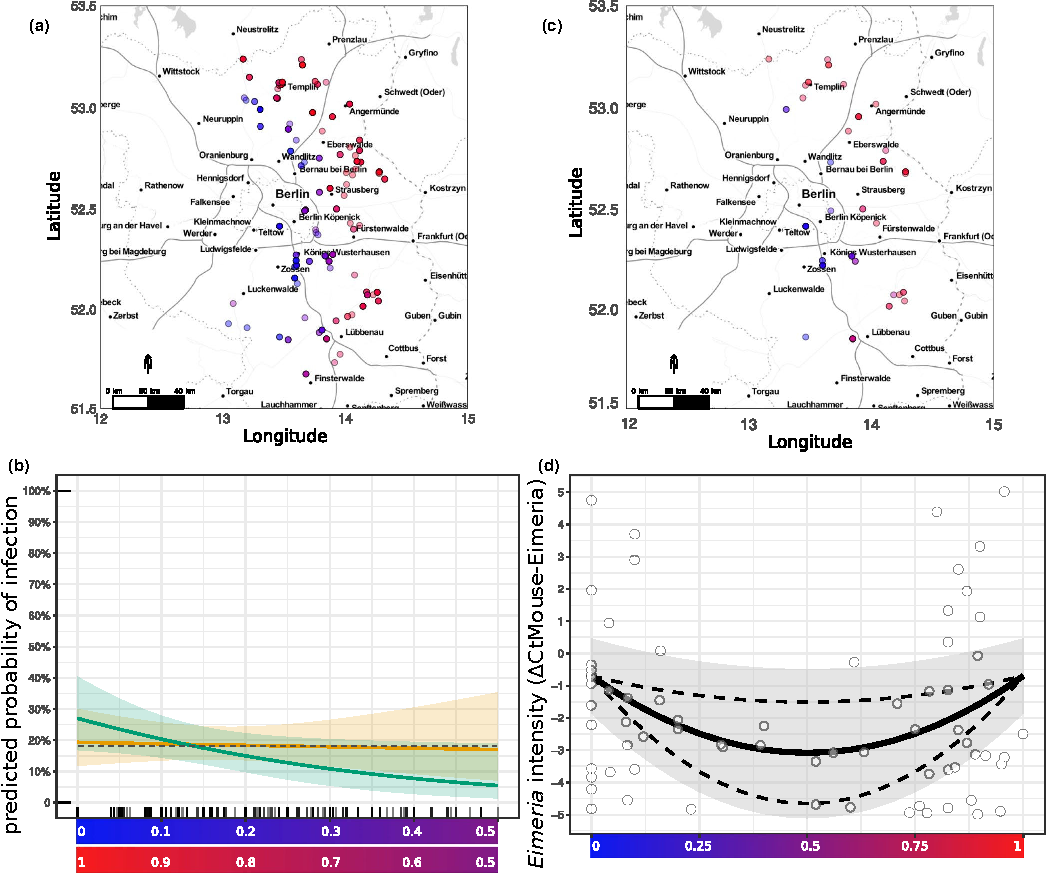
\includegraphics[width=\linewidth,height=\textheight,keepaspectratio]{images/2article1/Figure2.pdf}
    \caption{\textbf{Probability of infection is constant and intensity of \textbf{Eimeria} infection is reduced in hybrids}. Individual mice tested for detection and quantification of \textbf{Eimeria} spp. tissue stages (a) and mice tested positive (c) are displayed on a map (point color indicates mice genotype, on a gradient ranging from blue (pure Mmd) to red (pure Mmm); increasing number of mice sampled at one locality is displayed as decrease in transparency). The predicted probability of infection does not differ in more admixed mice (b) for males (green) and females (orange)(average overall observed probability of infection (prevalence) for males and females considered together: grey dotted line). \textit{Eimeria} intensity (white dots = individual mice) is reduced at intermediate values of the hybrid index (d), represented as a gradient ranging from 0 (pure Mmd, in blue) to 1 (pure Mmm, in red). The optimized fit is represented by a solid line, the 95\%CI of the fit as all parameters are allowed to vary in their 95\%CI, is plotted as a grey ribbon. The 95\%CI of the hybridization parameter alpha, as all parameters are fixed to their fitted value while alpha is allowed to vary in its 95\%CI, is plotted as dashed lines.}
\end{figure}

\subsection{\textit{Eimeria} spp. load is lower in infected hybrid vs pure Mmm and Mmd mice} 
To test more specifically the intrinsic host-parasite interplay of hybrids compared to pure mice, we considered only individuals infected by \textit{Eimeria} spp. tissue stages (N = 70). Complex models involving differences between sexes (H2 vs. H0 G-test: χ23 = 6.12, P = 0.89; H3 vs. H1 G-test: χ24 = 8.09, P = 0.91) and parental taxa (H1 vs. H0 G-test: χ21 = 0.11, P = 0.26; H3 vs. H2 G-test: χ22 = 1.13, P = 0.43) did not fit the data significantly better than the null model (Supplementary Table S8). The fit involving the hybridization effect, however, showed significantly higher likelihood than the model without it (G-test: χ21 = 8e-4, P = 0.02). Infected hybrids had significantly lower load of \textit{Eimeria} spp. tissue stages than expected if the load was linear along the hybrid index, with a hybridization effect parameter alpha of 0.74 (\textbf{Figure 2.2d}, values of parameters of the fitted model given in \textbf{Table 2.1}). Considering only the more prevalent \textit{Eimeria} species, \textit{E.~ferrisi} , infected mice (N=44), we found similar results: no significant improvement of the model when differences between sexes (H2 vs. H0 G-test: χ23 = 4.24, P = 0.76; H3 vs. H1 G-test: χ24 = 6.63, P = 0.84) and parental taxa (H1 vs. H0 G-test: χ21 = 0.43, P = 0.48; H3 vs. H2 G-test: χ22 = 2.37, P = 0.69) were included and significantly higher likelihood of the model with hybridization effect than the model without it (G-test: χ21 = 5e-4, P = 0.02, hybridization parameter = 0.73; see \textbf{Supplementary Figure S2.6b}). 

\begin{figure}[H]
	\centering
	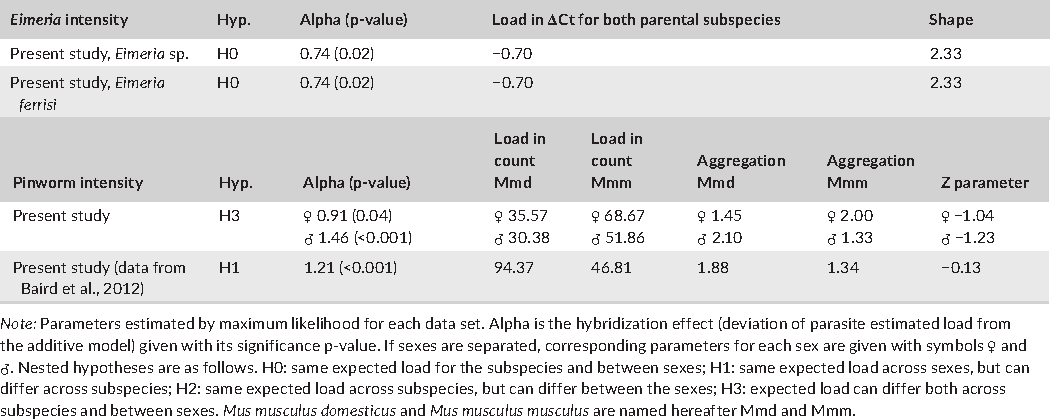
\includegraphics[width=\linewidth,height=\textheight,keepaspectratio]{images/2article1/Table1.pdf}
	\captionsetup{labelformat=empty}
	\caption{\textbf{Table 2.1.} Parametrisation of fitted models.}
\end{figure}
\addtocounter{figure}{-1}

\subsection{Pinworm load is lower in infected hybrid vs. pure Mmm and Mmd mice} 
We tested pinworm intensity (N = 307) in infected hybrids comparing them to infected “pure parental” mice in our Brandenburg transect, excluding potential ecological confounders in the same way. The model allowing differences between the parental taxa and sexes (H3) was found to fit our observations significantly better than the less complex models (H2 vs. H0 G-test: χ24 = 0.18, P = 0.004; H3 vs. H1 G-test: χ26 = 0.73, P = 0.006; H1 vs. H0 G-test: χ22 = 0.008, P = 0.004; H3 vs. H2 G-test: χ24 = 0.27, P = 0.008; Supplementary Table S8). For both sexes, the fit including the hybridization effect showed significantly higher likelihood than the model without it (females G-test: χ21 = 0.003, P =0.04; males G-test: χ21 = 3e-7, P<0.001). Infected hybrids had significantly lower pinworm load than expected if the load was linear across the hybrid index, with the hybridization effect parameter alpha 0.91 (females) and 1.46 (males) (\textbf{Figure 2.3d}, values of parameters of the fitted model given in \textbf{Table 2.1}).

\subsection{Comparison of pinworms loads with previous reports}
To compare the strength of the hybridization effect between our Brandenburg transect and the Czech-Bavarian portion of the HMHZ we applied the H1 model (differences between the taxa but not between the host sexes) to our pinworm abundance data, once with freely varying alpha (fit 1), and once with alpha set to 1.39 as in Baird et al. (2012) (fit 2). Within fit 1, alpha was found significant (G-test: χ21 = 1e-9 , P < 0.001). The comparison between the model with freely varying alpha (fit 1) and that using fixed alpha (fit 2) showed no significant likelihood difference (G-test: χ21 = 0.02, P = 0.11). Therefore, we can conclude that pinworm load differences found in hybrids in this study are consistent with the results obtained in the previously studied Czech-Bavarian transect \citep{baird_where_2012}. 

\begin{figure}[H]
    \centering
    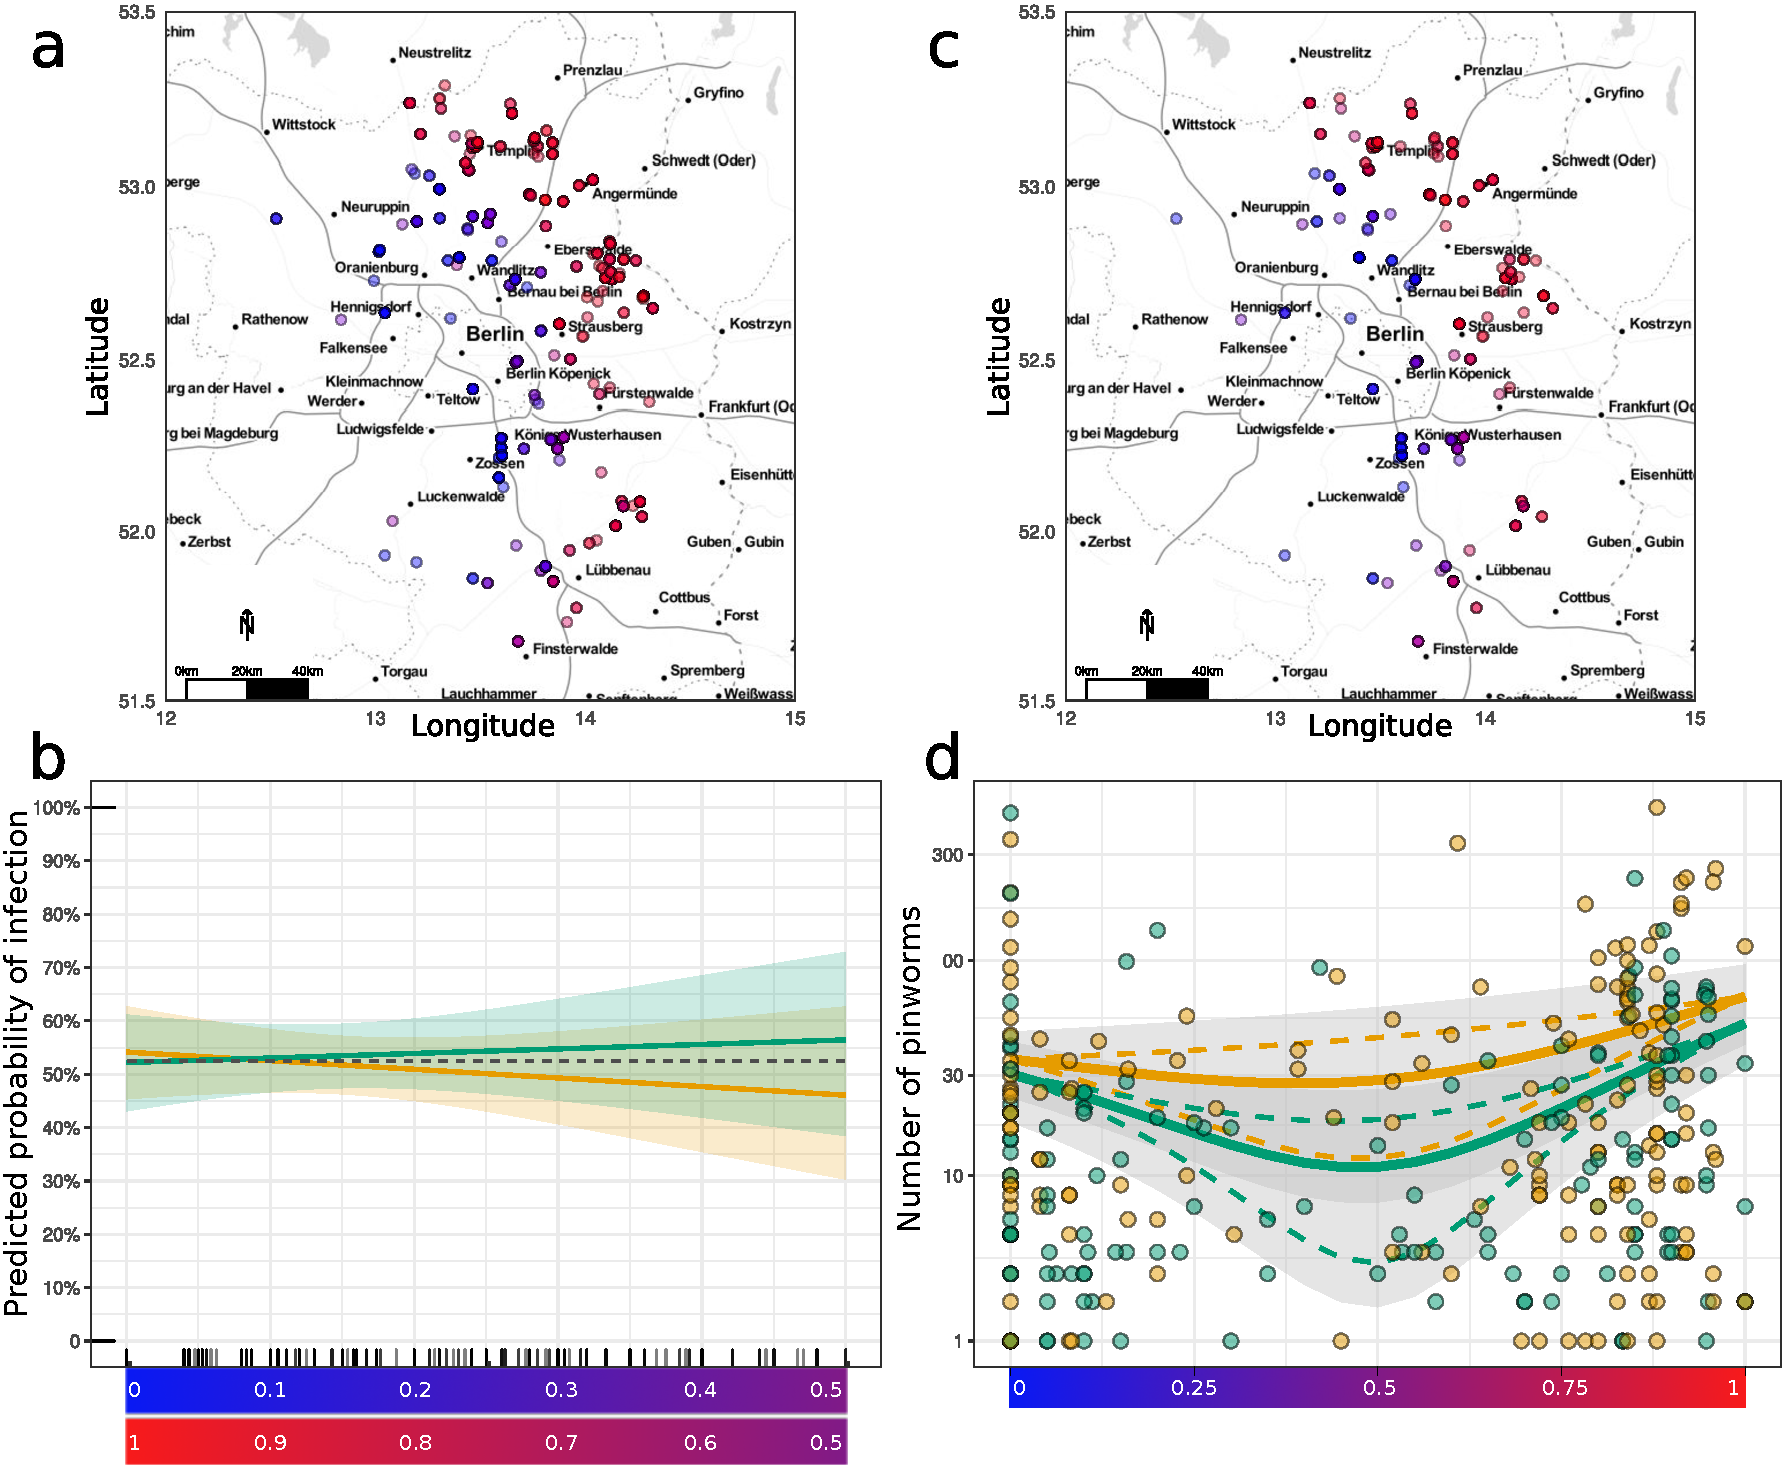
\includegraphics[width=\linewidth,height=\textheight,keepaspectratio]{images/2article1/Figure3.pdf}
    \caption{\textbf{Probability of infection is constant and intensity of pinworm infection is reduced in hybrids}.Individual mice tested for detection and quantification of pinworms (a) and mice tested positive (c) are displayed on a map (point color indicates mice genotype, on a gradient ranging from blue (pure Mmd) to red (pure Mmm); increased number of mice sampled at one point displayed as decrease in transparency). The predicted probability of infection does not differ in more admixed mice (b) for males (green) and females (orange)(average overall observed probability of infection (prevalence) for males and females considered together: grey dotted line). Pinworm intensity (white dots = individual mice) is reduced at intermediate values of the hybrid index (d), represented as a gradient ranging from 0 (pure Mmd, in blue) to 1 (pure Mmm, in red), for males (green) and females (orange). The optimized fit is represented by a solid line, the 95\%CI of the fit as all parameters are allowed to vary in their 95\%CI, is plotted as a grey ribbon. The 95\%CI of the hybridization parameter alpha, while all parameters are fixed to their fitted value and alpha is allowed to vary in its 95\%CI, is plotted as dashed lines.}
\end{figure}

\subsection{No evidence of body condition differences between infected and non-infected mice along the hybrid zone}
To test whether infections have a different effect in hybrids vs. parental mice we assessed body condition, which could be a better proxy for host health than parasite load. Modelling of the residuals from ordinary least squares regression of body weight by body length across the hybrid zone \textbf{Figure 2.4a} did not show a statistically significant hybridization effect in both parasite datasets considered (\textit{Eimeria} G-test: χ21 = 0.29, P = 0.41; pinworms G-test: χ21 = 2.81, P = 0.91). When infected and non-infected individuals were considered separately, neither \textit{Eimeria} spp. infected individuals (G-test: χ21 = 0.65, P = 0.58) nor \textit{Eimeria} spp. non-infected individuals (G-test: χ21 = 2.69, P = 0.90) showed a hybridization effect in body condition index \textbf{Figure 2.4b}. The same was true for pinworm infected individuals (G-test: χ21 = 0.34, P = 0.44) and pinworm non-infected individuals (G-test: χ21 = 4.12, P = 0.96; \textbf{Figure 2.4c}). 

\begin{figure}[H]
    \centering
    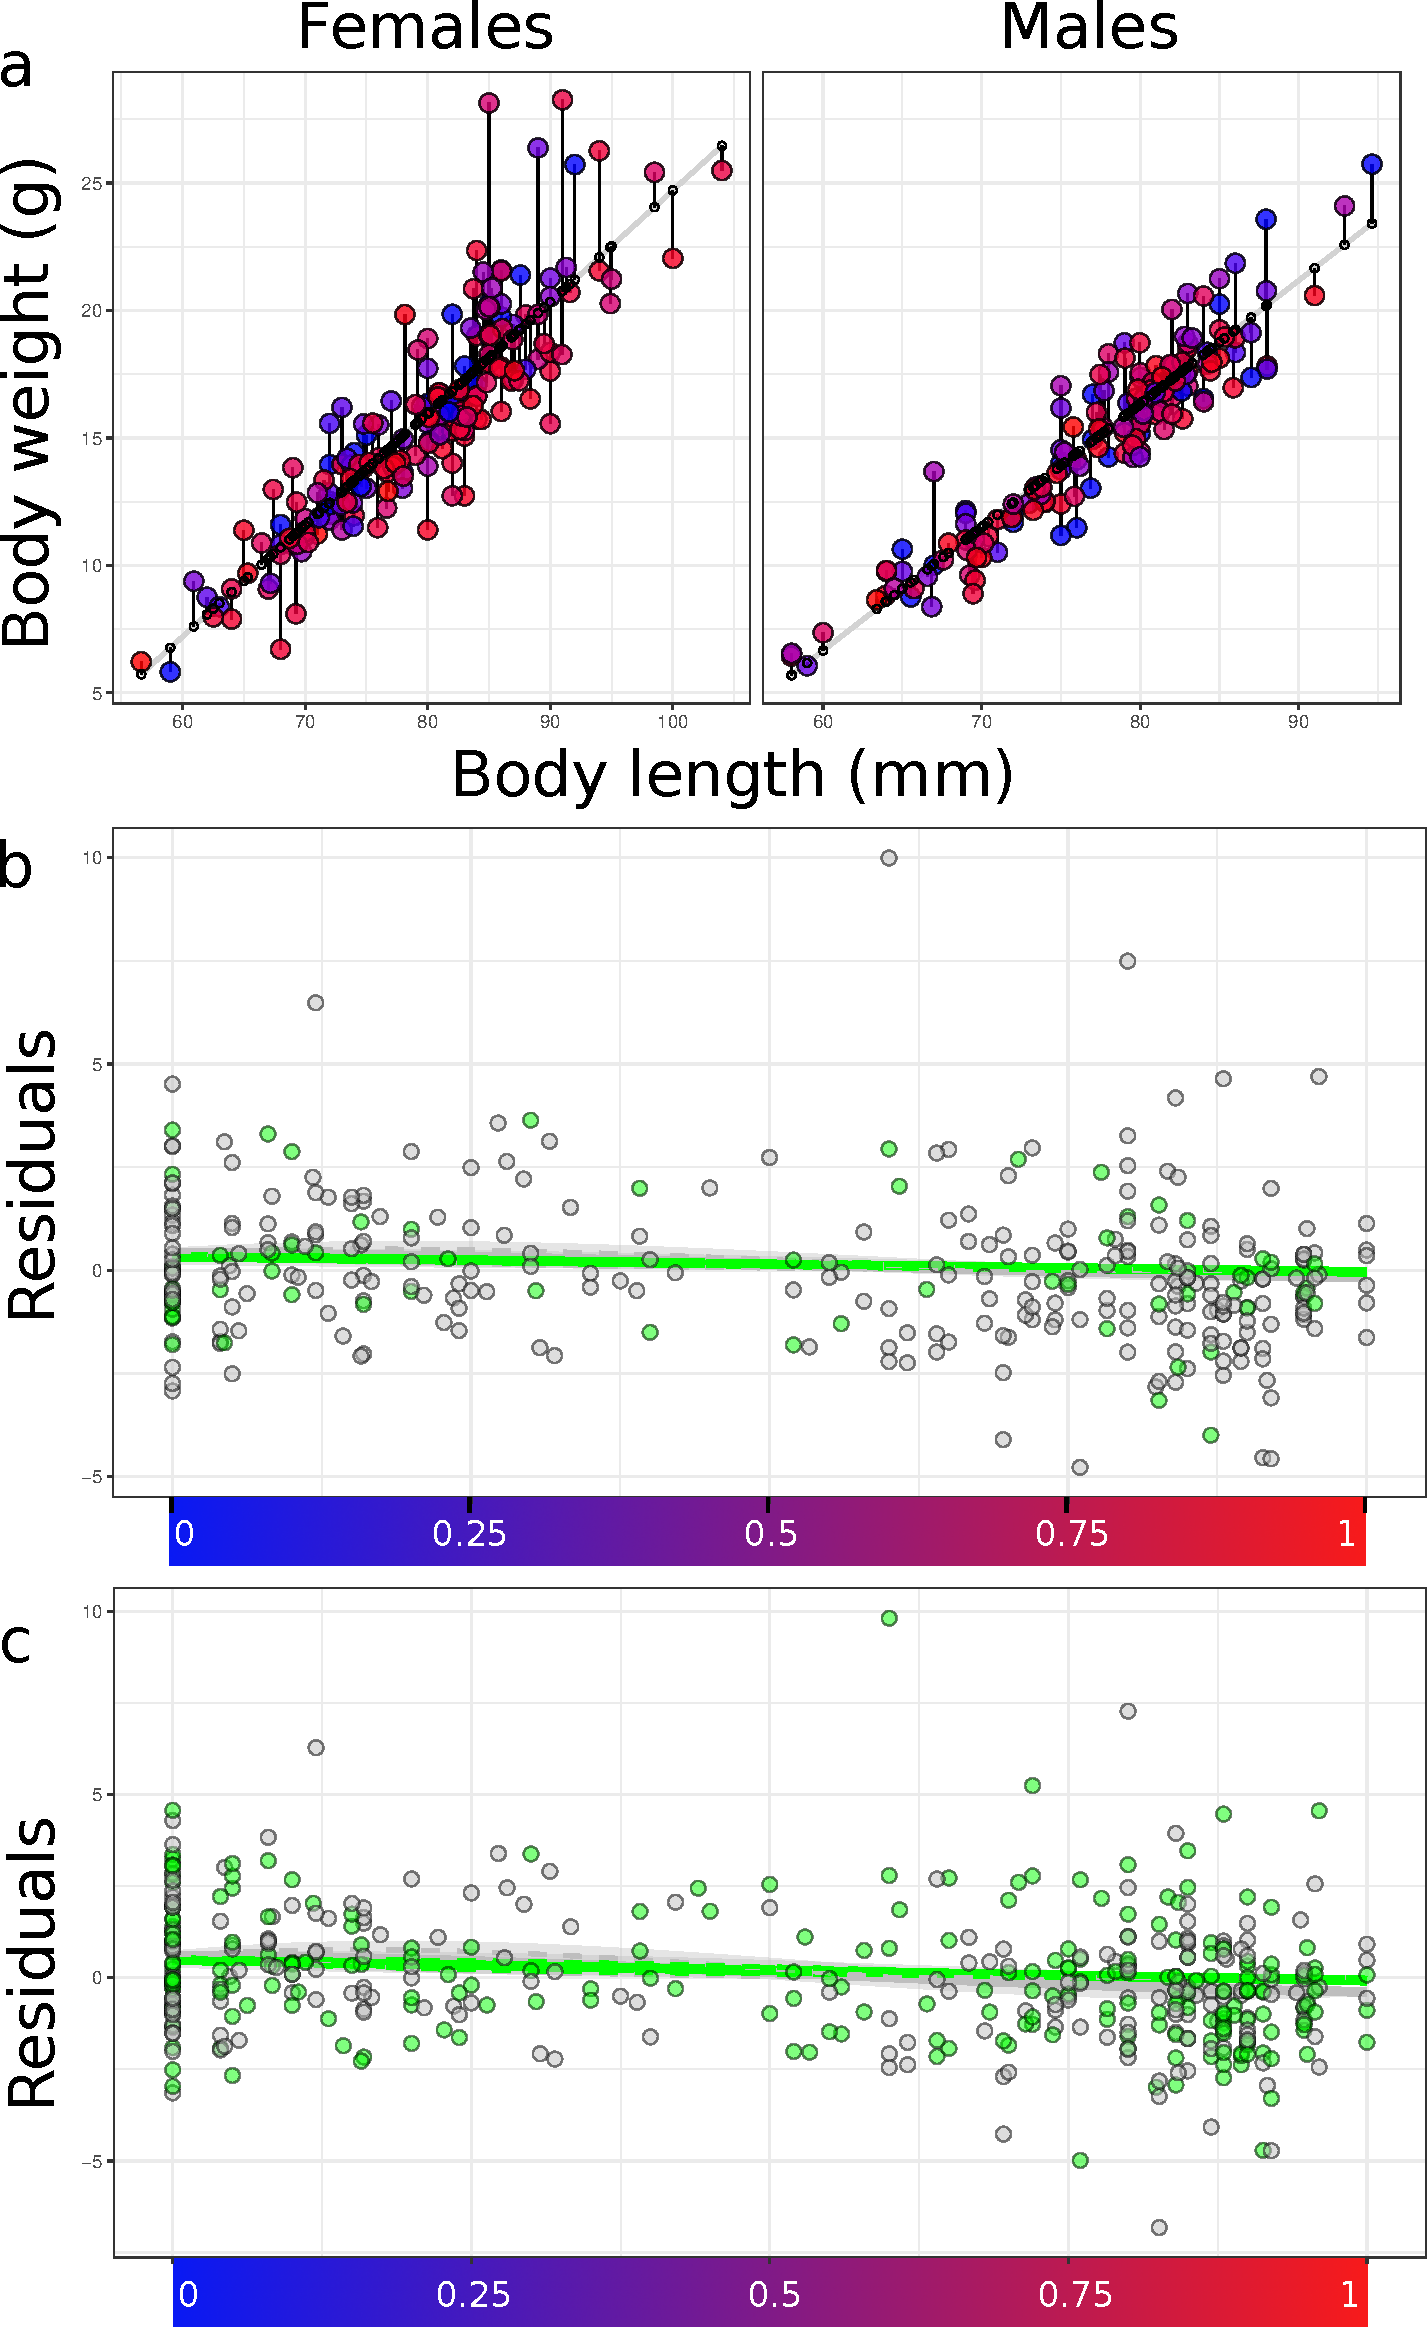
\includegraphics[width=.7\linewidth,height=\textheight,keepaspectratio]{images/2article1/Figure4.pdf}
    \caption{\textbf{Body condition does not significantly differ between hybrids and pure mice upon infection}. We modelled the residuals from ordinary least squares regression of body weight by body length along the hybrid zone. The fit and residuals for female and male mice is given in (a). The hybrid index is represented as a gradient ranging from 0 (pure Mmd, in blue) to 1 (pure Mmm, in red). ”Body condition” residuals along the hybrid index (for Eimeria spp. (b) and pinworms (c)) show no difference for infected mice (light green) and non-infected mice (grey). The optimized fit is represented by a solid line, the 95\%CI of the fit as all parameters are allowed to vary in their 95\%CI, is plotted as a grey ribbon. The 95\%CI of the hybridization parameter alpha, as all parameters are fixed to their fitted value while alpha is allowed to vary in its 95\%CI, is plotted as dashed lines.}
\end{figure}

\section{Discussion}
We found lower intensities of the intracellular parasites \textit{Eimeria} spp. and intestinal parasite pinworms in hybrid than in parental subspecies hosts in a previously unstudied transect of the European HMHZ. Lower intensity in hybrids is unlikely to be explained by ecological differences across the HMHZ, as we did not find the probability of infection to be similarly reduced in hybrid hosts, and no overall increase or decrease in mortality towards the zone centre. 
\par House mouse hybrids in the European HMHZ are not first-generation crossings, but rather genetically complex “late generation” recombinants. This means that each of their genomes presents a complex admixture of both Mmm and Mmd tracts \citep{macholan_genetic_2007}. There is no clear cut-off between hybrids and parental individuals. Therefore, individuals in such systems should not be considered in categories, but rather on a continuous scale of “hybridicity” (a hybrid index) when analyzing parasite infections or any other trait \citep{baird_where_2012}. We followed the statistical analysis of \cite{baird_where_2012} and explicitly modelled the effect of hybridization on parasite intensity by approximating the number of new combinations of genes brought together in a hybrid genotype by its expected heterozygosity (He). In other words we used He to derive non-linear predictions for hybridization effect based on the observed individual hybrid indices.  To increase reproducibility, we make our analysis available in an R package \citep{alice_balard_alicebalardparasiteload_2019}. The package allows statistical modelling with distributions additional to the original negative binomial distribution for (worm) count data \citep{baird_where_2012}. This allowed us to model the intensity of \textit{Eimeria} infections as measured by a recently established quantitative PCR \citep{ahmed_novel_2019, jarquin-diaz_detection_2019, al-khlifeh_eimeria_2019}.
\par To our knowledge no studies have previously tested the effect of mouse hybridization on parasites other than helminths in a field setting of the HMHZ. To understand the impact of immune diversity in hybrid hosts on parasites, it is necessary to test different types of parasites. Our parasite models present differences that are likely to involve different resistance mechanisms in their hosts (and also different impact on host health and immune systems, with intracellular parasites triggering mainly Th1 vs. extracellular parasites triggering mainly Th2 responses \citep{jankovic_th1th2_2001, maizels_parasite_1998}). Yet the pattern of reduced load in hybrid hosts is the same for the two parasites. These findings confirm that reduction in parasite intensity is either an effect intrinsic to the host individuals (e.g. enhanced immune reactions leading to increased resistance), or, if dependent on the parasite and/or parasite-host interplay, can be generalized over very different parasites. 
\par Adding more evidence to the original observations of reduced parasite loads for previously investigated parasites, we also found reduced pinworm loads in hybrids of our novel transect of the HMHZ. We found differences between the Brandenburg and Czech-Bavarian transects in pinworm infection such as distinct loads between males and females and lower prevalence (52.5\%) and abundance (18.7) in the former compared to the latter \parencite[no significant difference between sexes; prevalence 70.9\%, abundance 39.18;][]{baird_where_2012}. Geographical locations of the HMHZ likely present different ecological conditions underlying such differences. Despite this fact, the direction (lower intensity in hybrids) and strength of the hybridization effect were very similar in the two study areas. This similarity reinforces our confidence that reduced parasite load in mouse hybrids is a general phenomenon, intrinsic to the individual host genotype or host-parasite interplay rather than a by-product of ecology.
\par A novel aspect of our work compared to previous studies of parasitism in the HMHZ is the separate study of parasite prevalence and intensity. This approach should not only reduce problems in statistical inference caused by false negative measurements (so called zero-inflation) but also allows us to address two different questions separately: (i) Is the probability of infection different for hybrids and pure subspecies? and (ii): Is there a difference in parasite intensity between infected hybrid and infected pure individuals? 
\par An illustrative example of an ecological factor that could potentially lead to parasite load differences is the density of hosts. Densities of mouse populations in the HMHZ centre may be lower than outside \parencite[either due to selection against hybrids or because the HMHZ as a tension zone tends to be trapped in “density troughs” sensu][]{hewitt_sex-chromosome_1975}. Host density is expected to be positively correlated with pathogen transmission \citep{anderson_population_1979} and as a result prevalence may be higher in more dense populations \citep{morand_distribution_2000, hakkarainen_eimeria-parasites_2007}. This is, however, not a general law as host density and \textit{Eimeria} spp. prevalence are, for example, negatively correlated in bank voles \citep{winternitz_parasite_2012}. Independent of the direction of the effect, correlation between abundance and prevalence could be confounded with intrinsic effects of hybrid hosts.
\par Our analysis of prevalence (presence/absence in a logistic regression), did not however show any significant decrease of this probability of infection towards the centre of the zone, for neither \textit{Eimeria} spp. nor pinworms. Here we argue that, in conjunction with higher intensities, this distinguishes intrinsic hybrid effects from potential ecological confounders. 
\par Animals tolerant of low-pathogenic parasites might not suffer fitness reduction during high parasitemia. This could be the case, for example, if the parasite is beneficial for the host’s interaction with other parasites \citep{heitlinger_intestinal_2017} or if immune responses against the parasite are costly relative to the harm it causes \citep{raaberg_disentangling_2007}. In addition, according to the “Old Friend” (or “Hygiene”) hypothesis, the constant presence of helminths in natural populations has led to the evolution of a background basal release of regulatory cytokines \citep{rook_review_2009} which might in turn impact the outcome of more pathogenic infections. Even for relatively pathogenic parasites, such as \textit{Eimeria}, differences in resistance could be uncoupled from health effects by differences in tolerance \citep{raaberg_disentangling_2007}. For these reasons parasite load in itself should not be blindly considered as a proxy for host health and certainly not for host fitness comparisons across hybrid zones \parencite[see][]{baird_shifting_2019}. Here we used body condition as a proxy for the health component of host fitness. We, however, did not find evidence for differences in body condition between hybrids and pure mice upon infection. We conclude that we do not have evidence that lower parasitemia in hybrids increases their health. 
\par Intensity of a particular parasite infection is not necessarily correlated with reduced health and  fitness. For example, the fitness of sterile hybrids (always zero) is invariant to infection intensity. Moreover a hybrid host could be robust due to heterosis (though it may still be sterile). Even if we had found increased health of hybrids, this would not be interpretable as leading to a higher total hybrid fitness, as the parasite mediated health fitness component is only one (likely minor) component of overall fitness. It has been shown for example that male mice in the HMHZ centre have reduced fertility compared to parental individuals \citep{albrechtova_sperm-related_2012, turner_reduced_2012}. If reduced parasite intensity is host driven (and not a result of host-parasite interactions) one could conclude that some physiological systems (e.g. reproductive) may be more dependent on “co-adapted complexes”, while others – such as the immune system – benefit from diversity. This latter would be hybrid vigour in the narrow sense \citep{baird_where_2012}, but would still not necessarily lead to any effects on host species barriers \citep{baird_shifting_2019}. 
We can in future ask whether host (immunity and resistance), parasite (infectivity and virulence), or their interactions are underlying reduced parasite intensity in hybrid house mice. \textit{Eimeria} spp. are suitable pathogens to perform experimental and field studies in this endeavour. An experimental setup investigating resistance (inverse of parasite intensity) and tolerance (impact on host health measured by weight loss) during an infection in mice of pure subspecies and crosses between them could address this question in more detail.
\par A prime candidate locus for mediating a positive effect of hybridization on the immune system (hybrid vigour) is the major histocompatibility complex (MHC). In mice two genes of the MHC showed different levels of polymorphism as well as population structure with many alleles inferred to be shared between the subspecies by maintenance of ancestral polymorphism \citep{cizkova_genetic_2011}. Additionally, the small demes of house mice can function as reservoirs of MHC alleles, contributing to the diversity of this system across demes and populations \citep{linnenbrink_meta-populational_2018}. The genetic structure of the MHC and especially polymorphism shared across subspecies should make these loci good candidates to investigate for mechanisms behind hybrid vigour, among a number of other loci including Toll-like receptors \citep{skevaki_single_2015}. Previous work on toll-like receptor 4 already suggests different evolutionary patterns between the house mouse subspecies \citep{fornuskova_contrasting_2014}. For host parasite interactions major candidate loci are immunity related GTPases on the host side and rhoptry kinases in coccidia \citep{lilue_reciprocal_2013}. 
\par Hybridization has played a significant role during and after the divergence of house mouse subspecies as well as during the formation of “classical inbred strains” \citep{yang_subspecific_2011}. Improving our understanding of parasite process across the HMHZ provides valuable information on the house mouse as the (non-human) model species with the most thoroughly understood immune system. A transfer of knowledge from this model might further understanding of the interplay between parasites and hybridizing species, our own as well as species relevant for conservation.
